\section{Hierarchical VMO Generator}

\subsection{View model objects}

% introduction
The company's solution was developed in order to provide flexibility and customization to the end user. The middleware server retrieves all configurations from the metadata server. The configuration can be user specific information as well as global information e.g. the location of content distributors. The middleware translates the responses from the content distributors to Data Model Objects. They are the immutable objects that are transferred to the client's application. On the other hand, the client application operates with View Model Objects. They are used to render HTML pages. Single HTML page can contain single View Model Object. The VMO is constructed from multiple data model objects and some additional information (e.g. the location of the image).   

One important drawback can be observed: application duplication. The middleware server and the client application have the same pattern of execution: they both operate with data and build new data patterns from existing ones. The difference is that the middleware server is doing it with content distributor responses and the client aplication is processing middleware responses. Because of this situation, the client application should make several HTTP requests for retrieving necessary DMO objects from the middleware server.  The example of the single page generation is on picture \ref{fig:vmo_example}. As can be seen, in order to generate a single main page, the client application has to make about ten Ajax requests. What if there was a possibility to generate the VMO objects on the middleware side? Would there be a possibility to get rid of the duplication? What should be done for it? This section will describe the solution for removing duplication of MVC pattern and reducing the amount of requests to the middleware server. 

\subsubsection{VMO properties}

% describe examination of applications(Algar, RTelecom, ViaWeb)

Typical DMO and VMO objects are presented in Appendix E. As can be noticed, a VMO object is a JSON dictionary build from DMO objects. The VMO supports following properties:

Generic; The DMO objects are specific and unique for every content distributor. They are built according to the specific rules in the middleware server. The VMOs are generated from DMOs according to another set of rules specified in the client application. As a result in order to move VMO generation to the server side some descriptive language should be introduced that lets developers to describe the VMO structure.

Hierarchical; DMOs are basically data from content distributors. That means that the DMOs can be depend on other DMOs. For example, the figure [add DMO dep. figure] shows that in order to build a movie list DMO, first the DMO that represents movie categories should be generated, then for each movie category the set of movie objects should be fetched; Only on the third step can the list of movies be build. These means that the VMOs have a hierarchical structure. The typical VMO is presented in figure \ref{fig:vmo_example}.

\begin{figure}[h]
    \centering
	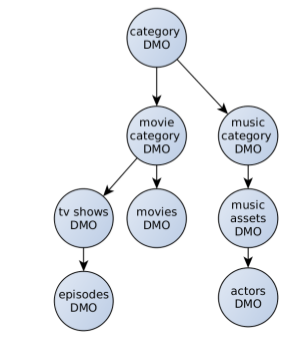
\includegraphics[width=8cm,height=10cm,keepaspectratio]{images/vmo_example.png}
    \caption{VMO from the set of dependent DMOs}
    \label{fig:vmo_example}
\end{figure} 

\subsection{Suggested Middleware server architecture}

In the current architecture, the single instance of the middleware server is deployed for a single content distributor. This is done due to the specifics of content distributors and data that they are providing. The following question arises: Is there a possibility to move the individual logic that requires to processes data to the client application while keeping the middleware as generic as possible? The theoretical benefits of this approach are: there will need to be a single middleware server or cluster deployed. This will simplify the deploying system; instead of supporting middleware for every content distributor, there will be just one. The new architecture is presented on figure \ref{fig:arch_overview_new}. As can be seen, the configuration server (Appgrid) is now treated like a content distributor. The benefit is that we do not need to specify separate logic for it. 

\begin{figure}[h]
    \centering
	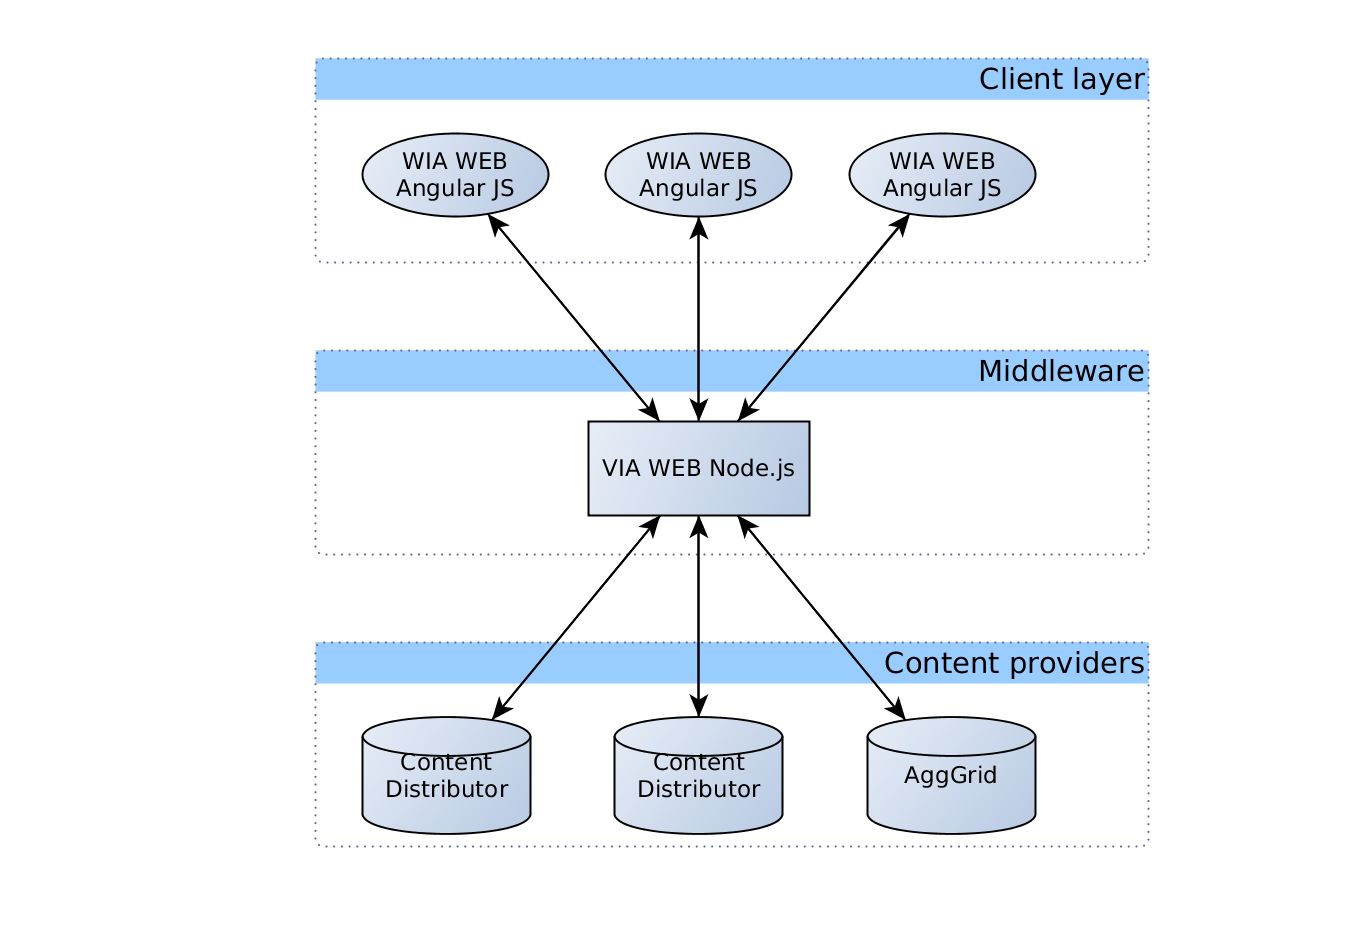
\includegraphics[width=\textwidth]{images/thesis_global_architecture_new.png}
    \caption{Manager workflow}
    \label{fig:arch_overview_new}
\end{figure}

Let's consider the architecture from another prespective.
The middleware server receives queries for the VMO generation. It supports several content distributors (databases) and makes queries to the content distributors for retrieving data model objects (tables). The middleware server resembles a relational database system. The comparison of database management system and middleware server is presented on figure \ref{table:db_ms}

\begin{table}
\begin{center}
  \begin{tabular}{||p{3in}|||p{3in}||}
    \hline
    Database & Middleware server VMO generation  \\ \hline
    serves multiple clients & should serve multiple client applications  \\ \hline
    supports creation of new databases & should support insertion of new content servers  \\ \hline
    supports creation and alternation of tables & should support creation and alternation of new endpoints  \\ \hline
    supports dynamic queries to the desired databases and tables & should support queries to the content distributors and their endpoints \\ \hline
    \hline
  \end{tabular}
  \caption{Comparison of Database System and Middleware Server properties}
  \label{table:db_ms}
\end{center}
\end{table}

\subsection{Approach description}

Let's consider relational database management systems and applications that are using them. Usually, there is a single instance or cluster of databases installed and deployed on servers, depending on the amount of requests it should serve. Nobody makes a new database instances for a single client, because it is neither efficient nor effective. In order to get data from the database the queries are executed. The SQL queries are basically the rich descriptive language that is interpreted by the database and executed for specified tables. The data is provided in two forms: array of table rows and array of view rows. Tables are the single source of information that resembles DMO. Views are the mixed information from tables that looks like VMO. 

In order to solve the problem of duplication and reduce the amount of requests, the hierarchical VMO generator(HVG) was developed. The HVG is basically the descriptive language that developers are writing in a JSON format. The JSON is then translated into the GET HTTP or POST HTTP request and sent to the middleware server. The middleware server parses the request, builds the asyclic graph, and fetches the corresponding data model objects. The data model objects are then combined together and sent as a response to the client application. The client application executes specific logic on the data received from server and builds HTML pages.

% The picture [insert picture] describes the VMO 

% picture of DBMS and Middleware server
% picture of DBMS tables and queries to the middleware server

\subsection{Path in VMOs}

This section introduces the definition of path in the View Model Object. The main format for data transferring is JSON. The JSON format consists of two main objects: array and dictionary. An example of dictionary:

\lstset{ %
    caption=The example of JSON dictionary,
    basicstyle=\ttfamily\footnotesize\bfseries,
    linewidth=0.6\textwidth
 }
\begin{lstlisting}[linewidth=5cm]
	{key1:value1,key2:value2,key3:{key1:value1}}
\end{lstlisting}

 
An example of array: 

\lstset{ %
    caption=The example of JSON array,
    basicstyle=\ttfamily\footnotesize\bfseries,
    linewidth=0.6\textwidth
 }
\begin{lstlisting}
	[value1,value2,value3:{key1:[value1,value2]}]
\end{lstlisting}

Very complex entities can be built using combinations of these two objects. Let's introduce the definition of path: The path is the route to the specific object or a set of objects in a JSON entity. 
The examples of path are presented below:
\lstset{ %
    caption=The examples of objects in different routes,
    basicstyle=\ttfamily\footnotesize\bfseries,
    linewidth=0.6\textwidth
 }
\begin{lstlisting}[linewidth=5cm]
	Object: {root:{child:value}}
	Path: root.child
	Value: value

	Object: {root:[{key:key1, value: value1},{key:key2,value:value2}]}
	Path: root.key
	Value: [value1,value2]

\end{lstlisting}


As can be seen, the path identifies a single object if it lays though a set of dictionaries. However, if the array is found on the route, all elements will be traversed and a set of objects will be extracted. 


\subsection{Hierarchical VMO Generator overview}

In order to solve the problem of multiple requests and middleware server duplication, the descriptive hierarchical VMO generator is implemented. It consists of three modules: HVG fetcher, HVG query parser, and HVG query builder. In order to build and process VMOs, two data structures are used: content provider dictionary and query dictionary. 

The content provider dictionary has a tree-based structure and its scheme is presented on \ref{fig:content_provider_map}. Rectangles indicate the single instance of object appends, while parallelograms indicate the dictionary of objects. The content provider dictionary contains a dictionary of content distributors. When the query is passed to the middleware server, the locations of necessary content distributors are retrieved from this dictionary. It is used by the HVG fetcher module.

The key is a unique identifier that is used by query objects (as described below). Each content provider consists of two parts: location and a dictionary of resources. The location is a domain with corresponding scheme. The resource has one field: endpoint. The endpoint is a path in URI [RFC to URI] with several embedded templates. The template can be one of two types: \textit{\{param\_id\}} and \textit{\{param\_id*\}}. The first type indicates that only one value can replace the template. If an array of values is given, it will produce the array of resolved endpoints. On the other hand, the second type produces a single endpoint, even if an array of values is given. The examples of templates are presented in table \ref{table:template_replacement}.

% TODO: purpose

\begin{table}
	 \begin{center}
	  \begin{tabular}{l l}
	    Input values: & \textit{\{id:[value1,value2,value3]\}} \\
	    Endpoint: & \textit{http://testdomain.ext/\{id\}}  \\ 
	    Result: & [\textit{http://testdomain.ext/value1}   \\
	    		&  \textit{http://testdomain.ext/value2}   \\
	    		&  \textit{http://testdomain.ext/value3}]  \\
	    Endpoint: & \textit{http://testdomain.ext/\{id*\}} \\
	    Result: &  \textit{http://testdomain.ext/value1,value2,value3}
	  \end{tabular}
	 \label{table:template_replacement}
	 \caption{URL Template examples}
	\end{center}
\end{table}

The example of content provider map is given in Appendix C.


\begin{figure}[h]
    \centering
	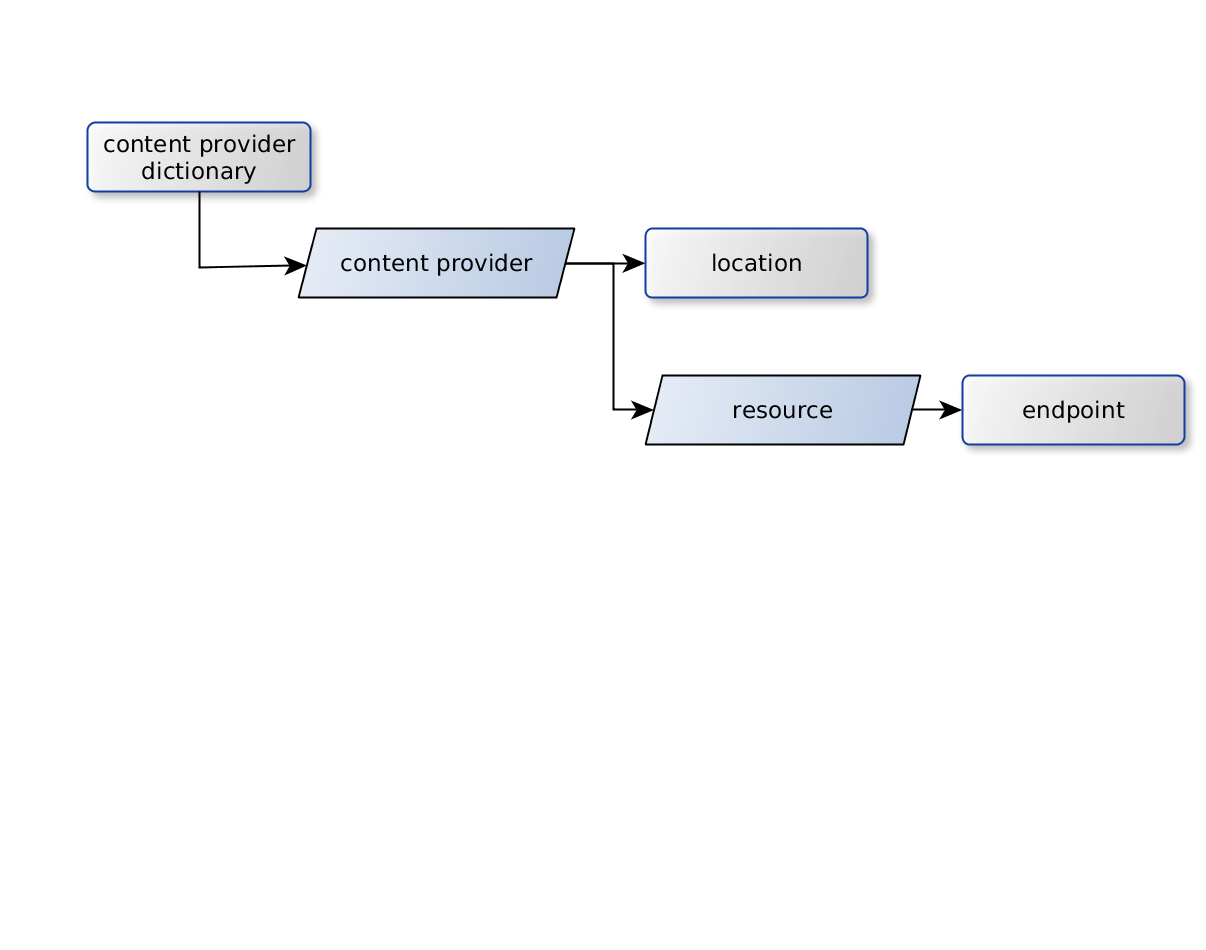
\includegraphics[width=\textwidth]{images/content_provider_map.png}
    \caption{Content Provider dictionary structure}
    \label{fig:content_provider_map}
\end{figure}


The query represents the request from the client application to the middleware server. The tree-based structure is presented on figure \ref{fig:query_structure}. The single query consists of several query objects.

The query is built on the client application using HVG query builder. When the query is finished, it is translated into a corresponding JSON format and sent to the middleware server.

Each query object may have up to three parameters: \textit{content\_distributor}, \textit{path\_parameters}, \textit{query\_parameters}. The obligatory parameter, or \textit{content\_distributor}, corresponds to the key in the content provider dictionary desrcibed above. Through it, the set of resources is retrieved from the content provider dictionary. The \textit{path\_parameters} and \textit{query\_parameters} are similar to each other, as a result only one of them will be described. The \textit{query\_parameters} is a dictionary of parameters, the key corresponds to the template parameter in resource object described above. Each path parameter has a type field. It can have one of two values: \textit{constant} or \textit{dependency}. If the value is \textit{constant}, only one additional field should be specified: \textit{values}. This field serves as a container of values that should replace the corresponding template in the endpoint. 


On the other hand, if the value of \textit{path\_parameter} is \textit{dependency}: the query object depends on another query object (e.g. when getting the list of movies from the content distributor), the list of categories should be requested first. That means that in order to request a query object, the parent object should be requested first and then the specified dependency variables for the template parameters should be retrieved. In this case, additional parameters should be specified: \textit{parent}, \textit{parent\_parameter\_type}, \textit{path} and \textit{property}. The \textit{parent} specifies the query object identifier of the parent object. The \textit{path} is a JSON path to the object as described above. The \textit{property} is a key in the dictionary retrieved by using \textit{path} parameter. The \textit{parent\_parameter\_type} can be one of two values: \textit{key} or \textit{constraint}. If the value is \textit{key} then the dependency variables will be extracted using path: \textit{path}+\textit{property}.

If the value of \textit{parent\_parameter\_type} is \textit{constraint} then the objects in \textit{path} that obey constraints will be retrieved. In this case, the additional parameter should be specified in corresponding path parameter: \textit{constraints}. The \textit{constraints} is an array of constraints. Each constraint has two parameters: key and value. The key specifies the name of the property that the object should have and the value specifies the value of the property. The summary of parameters is presented in the Table \ref{table:query_obj_desrc}.


\begin{center}
	\begin{table}
	  	\caption{Description of Query Object's parameters}
	 	\label{table:query_obj_desrc}
	  	\begin{tabular}{|l|p{4in}|}
	    \hline
	    Parameter & Description  \\ \hline
	    content\_distributor & the location of resource dictionary in provider  \\ \hline
	    path\_parameters & dictionary of variables that will be retrieved in runtime and replace the corresponding template parameters in endpoint for building a request URL  \\ \hline
	    type & the type of path\_parameter, can be constant or dependency  \\ \hline
	    parent & the parent ID of query object. Note: specified only when type=dependecny \\ \hline
	    parent\_parameter\_type & the parent parameter type, can be key or constraint. Note: specified only when type=dependency \\ \hline
	    path & the path for the objects in parent response. Note: specified only when type=dependency \\ \hline
	    property & the name of property that contains dependency value. Note: specified only when type=dependency \\ \hline
	    constraints & the array of constraint. Note: specified only when type=dependency  and path\_parameter\_type=constraint\\ \hline
	    \hline
		\end{tabular}
  	\end{table}
\end{center}


Hierarchical Query Parser(HQP) is a module that translates client requests into JSON format. The available methods are presented in table \ref{table:hqp_parameters}.

\begin{center}
	\begin{table}
		\label{table:hqp_parameters}
	  	\caption{Description of HQP module}
		\begin{tabular}{|l|p{1in}|p{3in}|}
	    \hline
	    Method Name & Parameters & Description  \\ \hline
	    select & object ID, content distributor ID & creates an empty query object with specified content distributor ID  \\ \hline
	    setConstantParameter & parameter ID, values & appends the path parameter which has a type \textit{constant} to the query object's path\_parameters dictionary  \\ \hline
	    setParentParameter & parameter ID, parent query object, path , property & appends the parent parameter to the query object  \\ \hline
	    setQueryParameter & key, value & appends query parameter to the query objects query\_parameters dictionary \\ \hline
	    addConstraints & path parameter ID, array of constraints& appends the constraint array to the query object's path patrameter \\ \hline
	    build & &  translates query objects into JSON format  \\ \hline
	    \hline
	  	\end{tabular}
  	\end{table}
\end{center}

The example of HQP usage is given in Appendix D.


\begin{figure}[h]
    \centering
	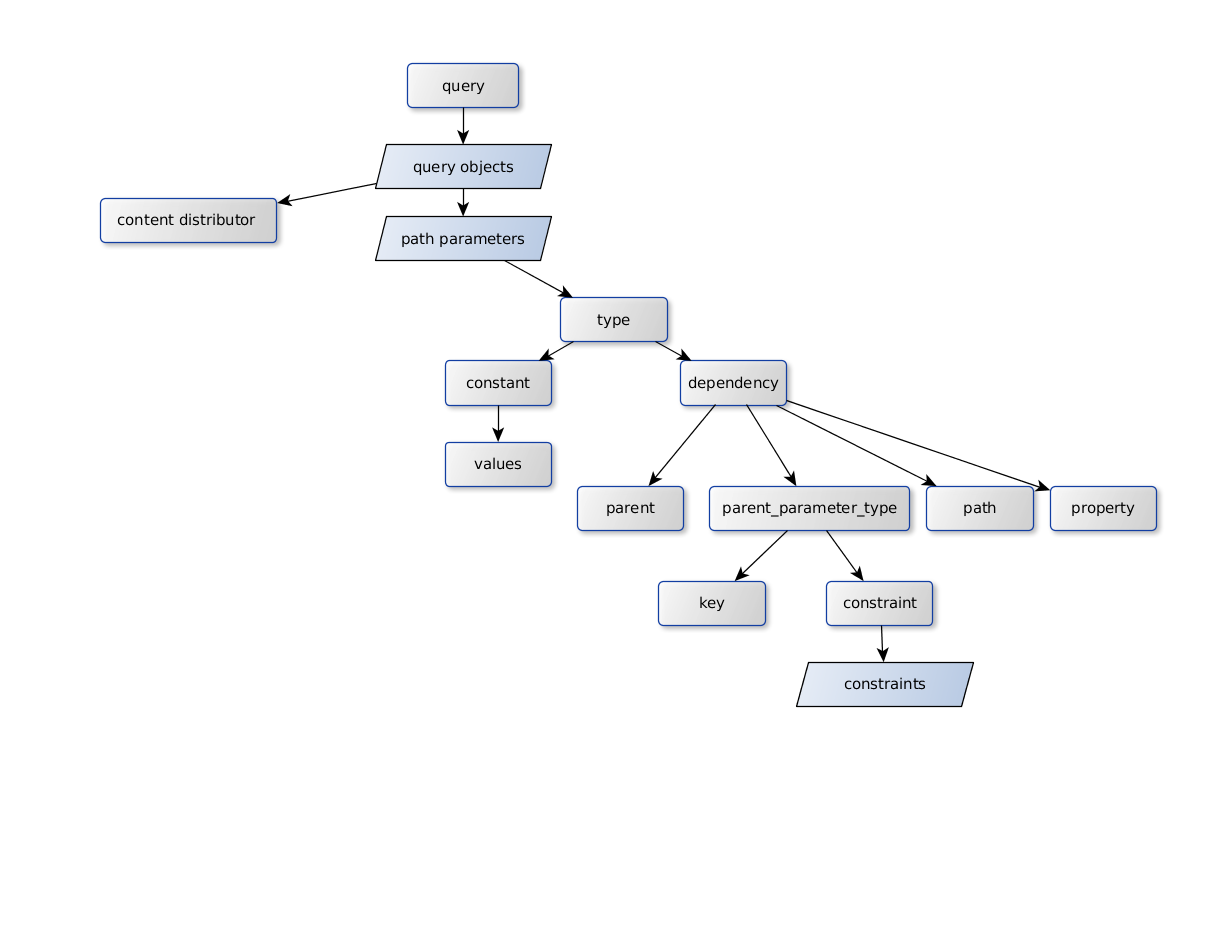
\includegraphics[width=\textwidth]{images/query_structure.png}
    \caption{Query structure}
    \label{fig:query_structure}
\end{figure}


The HQL supports two level caching. The first level caches the data model objects. It lays after parsing the client request strictly before requesting data from the content distributor. The second level cache lies on top of the execution process and is touched before executing the client request.  

% TODO: add section about asynchronous computation

\subsection{HQL workflow}

The developer writes the request using HQL parser methods. The request is translated into a JSON format that contains a dictionary of query objects. The JSON is sent as a POST HTTP request to the middleware server. The middleware server builds the asyclic graph (if there were dependency cycles it will generate error). The direct asyclic graph is then traversed using breadth first search algorithm, on every node (query object) the data is fetched from the appropriate content distributor (if the parent data has already been fetched) and is written into the output array. The output array is then sent as a response to the client POST request. 

The schematic workflow of HQL fetcher and HQL query parser is presented on fiqure \ref{fig:hvg_workflow}.

\begin{figure}[h]
	\begin{center}
		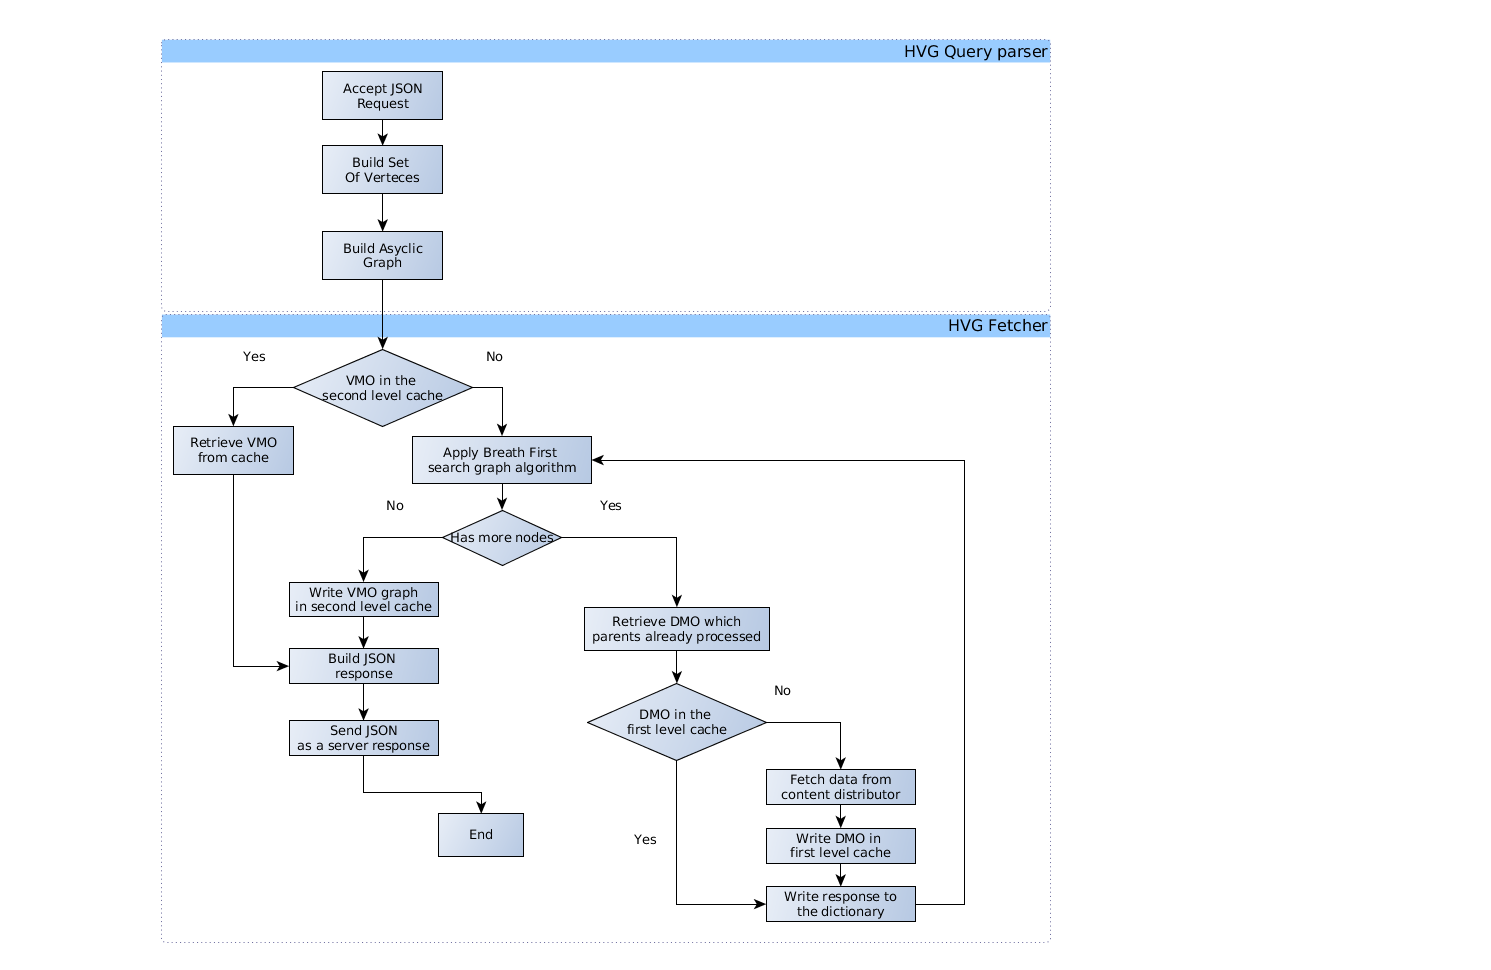
\includegraphics[width=20cm]{images/hvg_qp_workflow.png}
   		\caption{HVG workflow}
    	\label{fig:hvg_workflow}
	\end{center}
\end{figure}

\subsection{Alternatives to HVG}

The middleware server can be used in order to build one of three object types: Data model object, View model object or Application model object. The initial implementation was responsible for building DMOs. The current implementation builds the VMOs.

The DMO and VMO were described above. The Application Model Object(AMO) contains a set of VMOs that are specific for a content distributor. The alternative to the dynamic VMO generation on the middleware side can be a generation of AMOs on the middleware server. However, it is not a good idea because the size of object provided by content distributors can vary a lot and some of them can be very heavy. If the full AMOs would be transferred to the client application, a big amount of memory would have to be utilized by both client application and middleware server. In theory, it will dramatically decrease the user experience, but it could be checked as a continuation to this project.


\newpage